\section{Prediction for unassociated sources in 3FGL and comparison with 4FGL}
\lb{sec:3FGLprediction}


In this section we use the selected algorithms from the previous section to predict classes for the unassociated sources in the 3FGL. 
We then use the associations, which exist for some of these sources in the 4FGL, to check the accuracy of our methods on the unassociated data.  A total of 242 such sources were identified for which we could find associations. All of these sources have an FGL counterpart name in the 4FGL. There were also those which had an FHL counterpart name, but we ignored them for the purpose of this study.\\
%\subsection{Unassociated sources in 3FGL with associations in 4FGL}
%There were a total of 286 sources without associations in 3FGL but associations in 4FGL. We trained our algorithms on the entire set of associated data from the 3FGL, and then tested our algorithms on these 286 sources. The probabilistic version is discussed in the next section.  \\

Accuracies of our chosen algorithms are given in table 2, averaged over 1000 runs. It contains both intial test and comparison testing accuracies, where comparison now refers to the 3FGL unassociated data with associations in 4FGL. 


\begin{table}[!h]

\resizebox{0.45\textwidth}{!}{
    \tiny
 %  \centering
    \renewcommand{\tabcolsep}{0.3mm}
\renewcommand{\arraystretch}{1.5}

    \begin{tabular}{|c|c|c|c|}
    \hline
    Algorithm&Parameters & Average  & Comparison \\
    & & Testing Accuracy & with 4FGL accuracy\\
    \hline
    RF& 50 trees, max depth 6  &97.42& 97.19  \\
    \hline
    NN & 300, 10 Neurons, Adam & 97.40& 95.65 \\
    \hline %\midrule   -> aakash do you mean this?
    BDT & 100 trees, max depth 2    &   97.80&96.28 \\
%    \hline %\midrule   -> aakash do you mean this?
%    BDT & 200 trees, max depth 2    &   95.8  \\
    \hline
    LR & LBFGS solver, 200 iterations & 97.60& 95.09 \\
    \hline
     
    \end{tabular}}
    \vspace{0.2cm}
    \caption{Accuracy of the 4 selected algorithms on 3FGL unassociated data.}
    \label{tab:selected_algs}
\end{table}

%As can be seen above, the best accuracies were found with less complicated models, which allowed bias to be low. The models were complicated enough to neither under, nor overtrain.

%Feature importance for RF: [0.         0.         0.12236186 0.31656891 0.12013348 0.04952569  0.05523149 0.05632573 0.23685429 0.04299855]



\subsection{3FGL Probabilistic classification} 

Here we discuss the results of our probabilistic classification on the unassociated data. The 242 sources for whom FGL counterparts existed were plotted in figure 10. This figure shows all AGNs and PSRs, including those which were correctly or incorrectly identified by all the 4 algorithms (given by keyword only) and those which are a mix of correct and incorrect classification by at least one of the 4 algorithms (given by keywords either/or). 
\begin{figure*}[h]
\centering
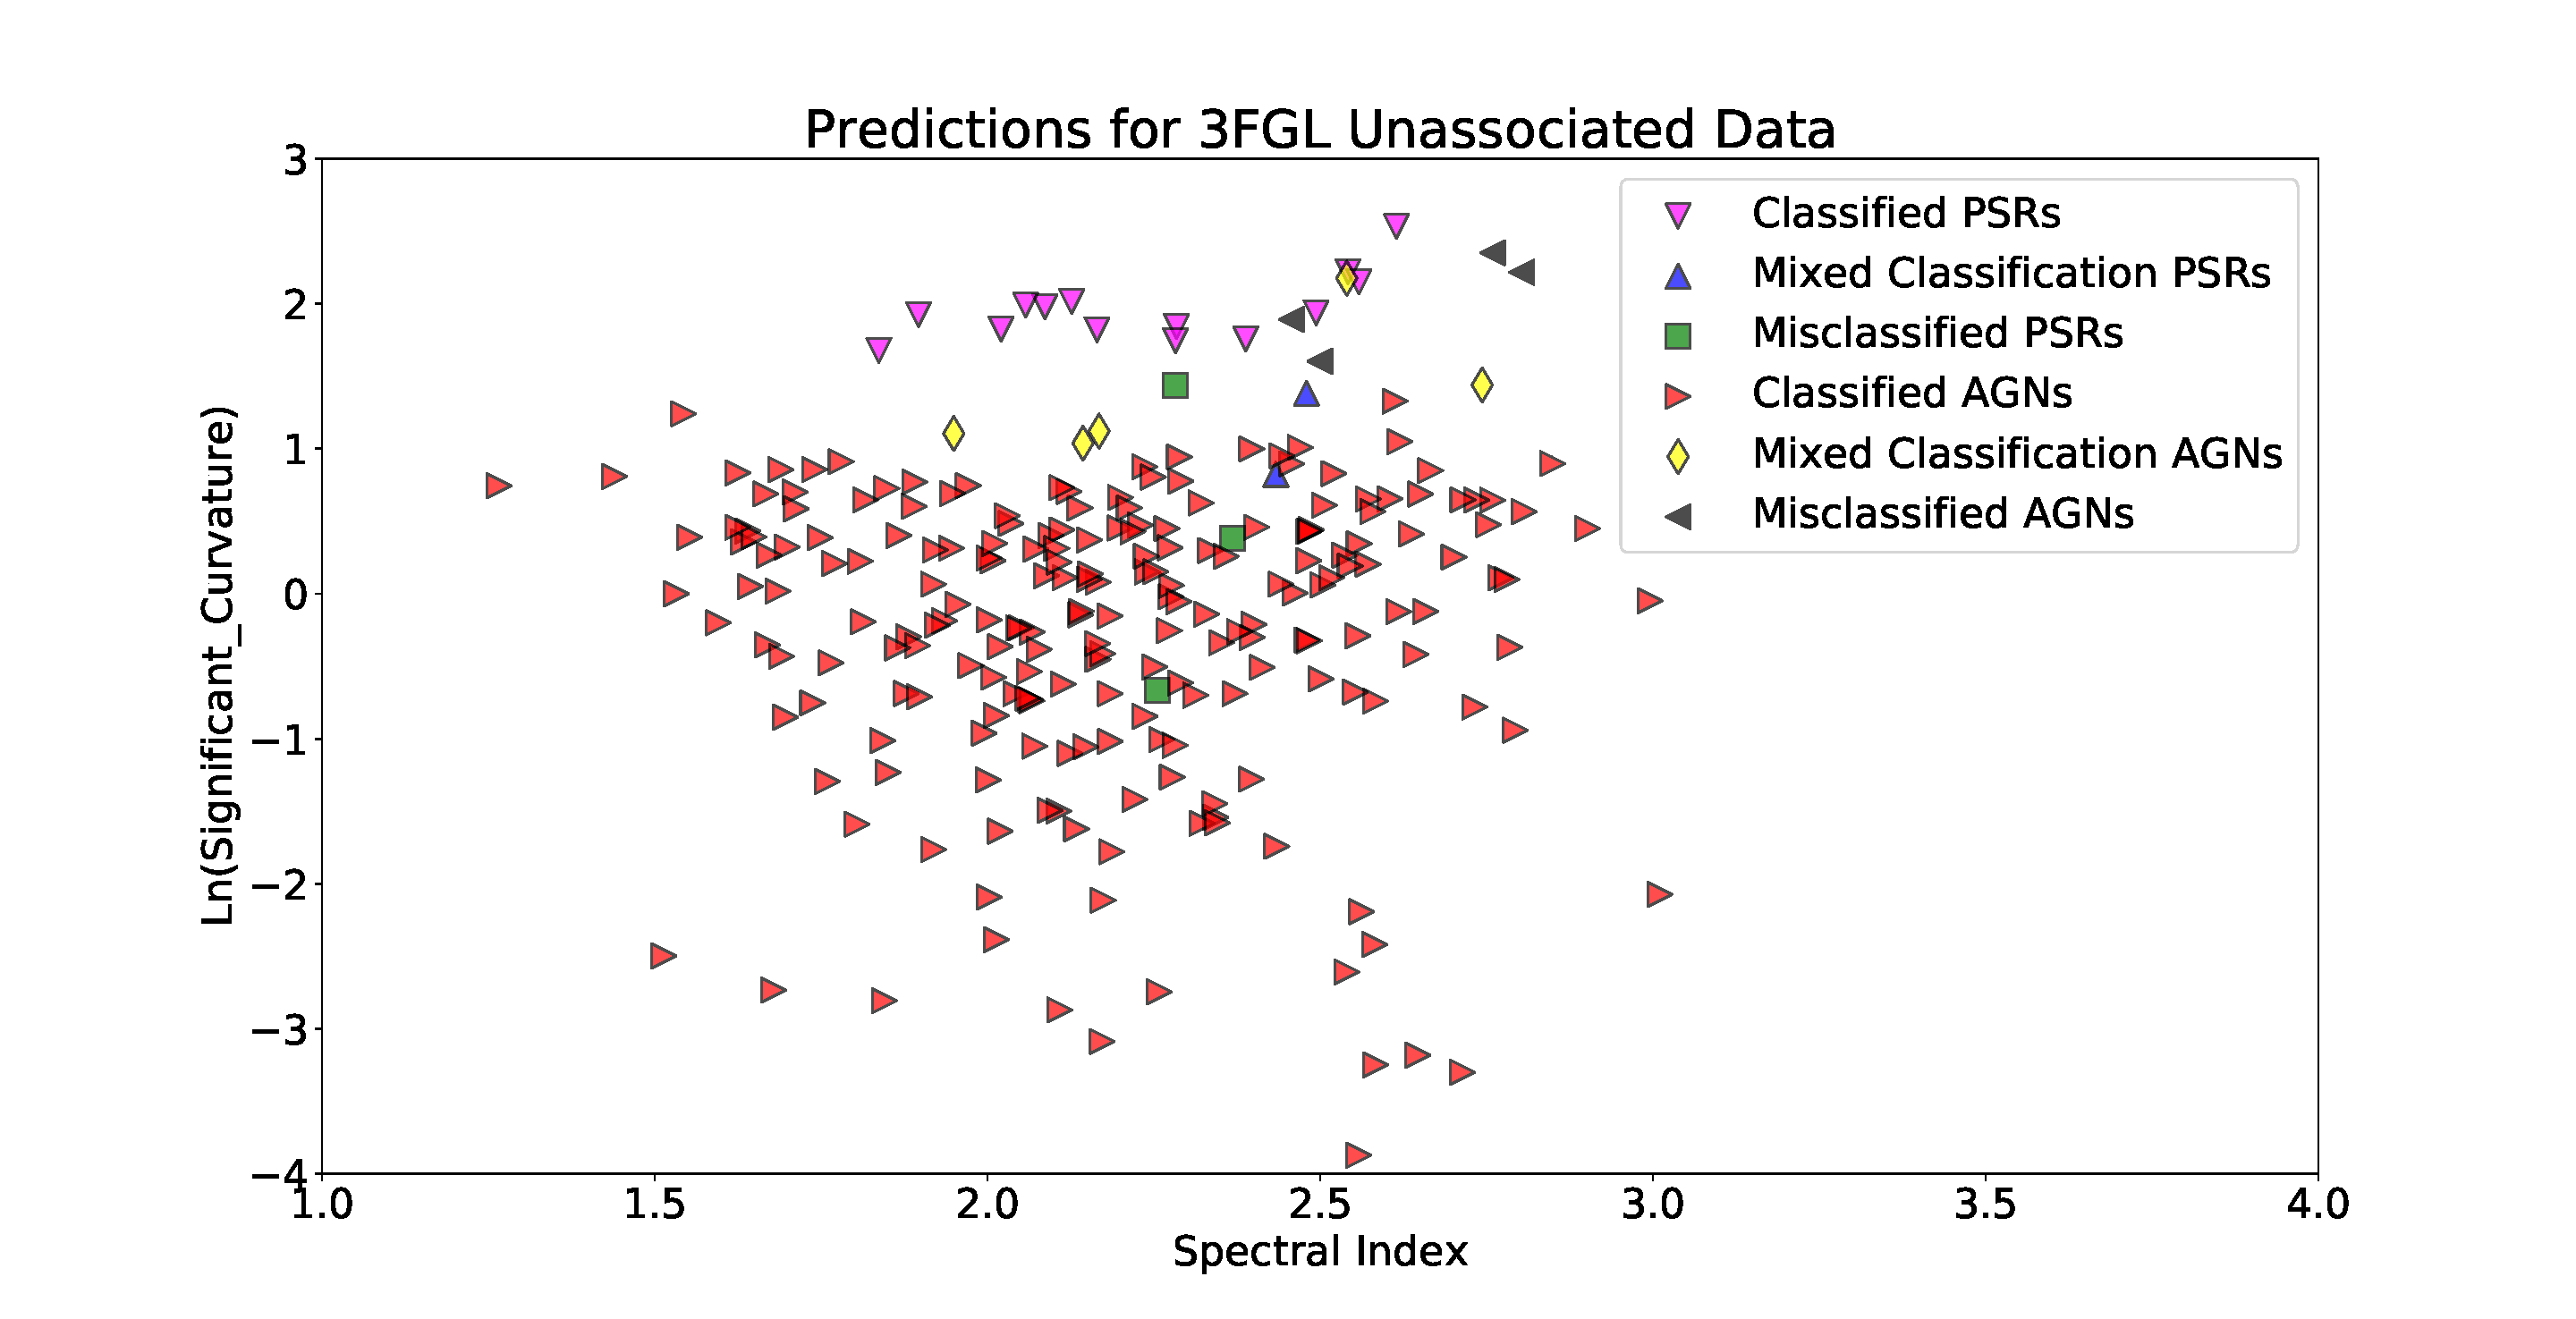
\includegraphics[width=\textwidth]{plots/plot_final.pdf}
%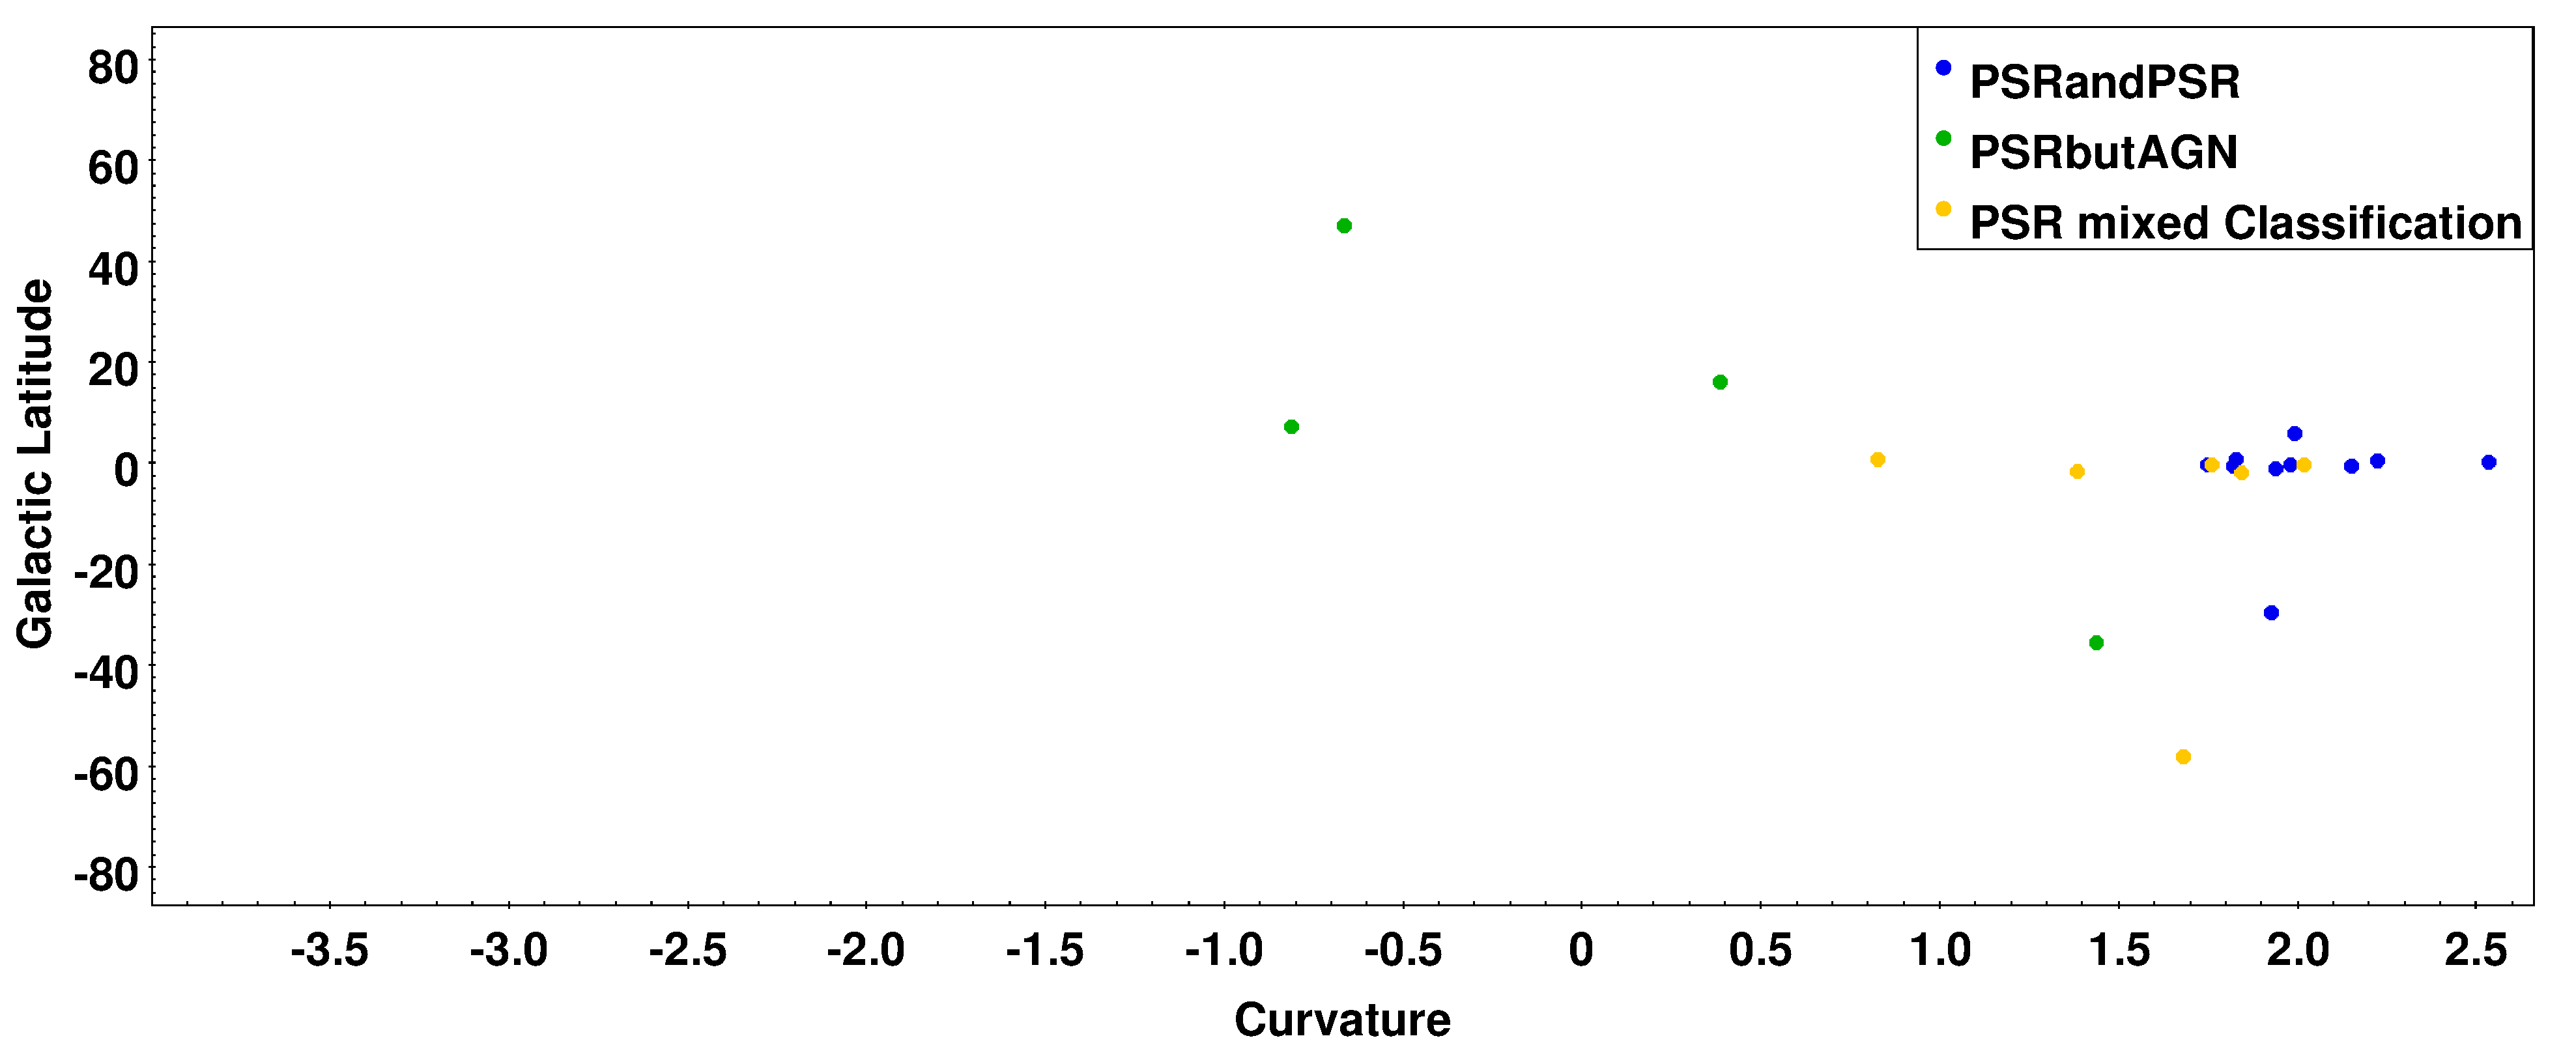
\includegraphics[width=\twopicsp\textwidth]{plots/PSR3.pdf}
\caption{Comparison of class prediction for unassociated 3FGL sources with classes in 4FGL. }
%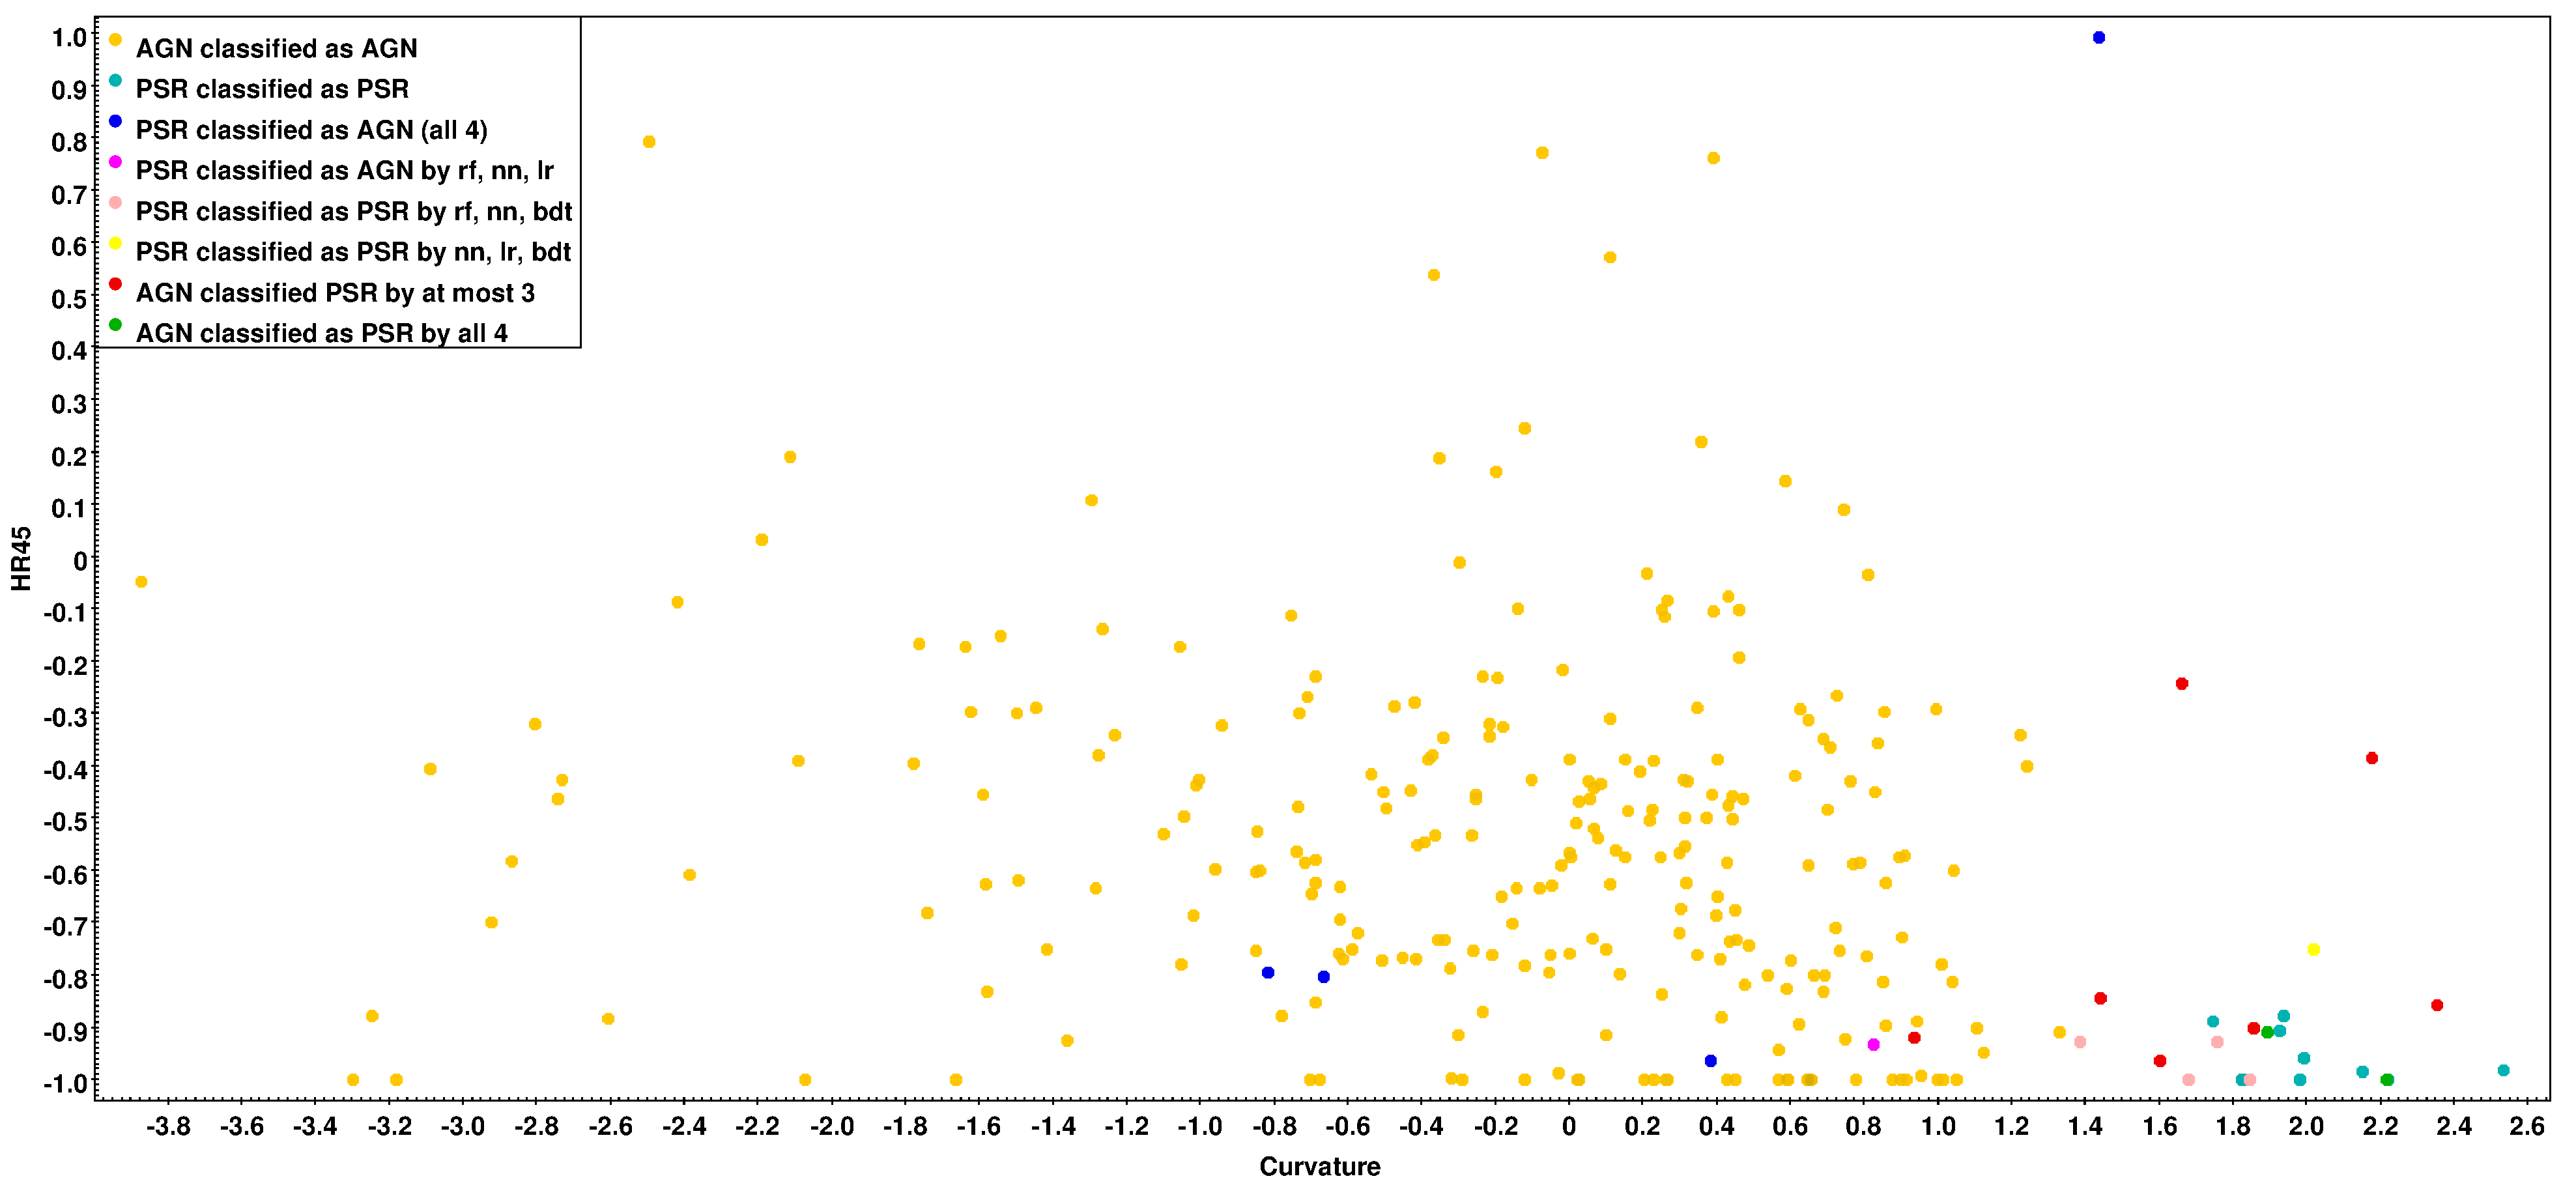
\includegraphics[width=\twopicsp\textwidth]{plots/final_catalog.pdf}
\label{fig:Maps_data}
\end{figure*}

%\csvreader[tabular=|l|l|c|,
  %  table head=\hline & Source Name &Flux \\\hline,
 %   late after line=\\\hline,
%filter={\value{csvrow}<2},]%%
%{data/3fglunassoc_4fglassoc_withprob.csv}{Source_Name_3FGL=\source,ln(Flux_Density_3FGL)=\flux}%
%{\thecsvrow & \source & \flux}

Table 4 shows an example of the probabilistic catalog we created for these 242 sources.

\pgfplotstableread[col sep=comma]{data/catalogs/3FGL_unassoc_vs_4FGL_assoc.csv}\loadedtable
\begin{table}
\pgfplotstabletypeset[columns={Source_Name_3FGL,AGN_BDT,AGN_RF,AGN_LR,AGN_NN},
column type=l,
string type,
every head row/.style={before row={\toprule & \multicolumn{4}{c}{AGN Probability} \\},after row=\midrule,},
every last row/.style={after row=\vdots },
%every first column/.style={column type/.add={|}{}},
%every last column/.style={column type/.add={}{|}},
columns/Source_Name_3FGL/.style={column name=Source Name},
columns/AGN_BDT/.style={column name=BDT,numeric type,fixed,precision=3},
columns/AGN_NN/.style={column name=NN,numeric type,fixed,precision=3},
columns/AGN_RF/.style={column name=RF,numeric type,fixed,precision=3},
columns/AGN_LR/.style={column name=LR,numeric type,fixed,precision=3},
skip rows between index={4}{242}
]\loadedtable
\caption{Catalog Rows and Columns for 3FGL unassociated data}
\end{table}
%\pgfplotstabletypeset[
%    col sep=comma,
 %   string type,
%table head=\hline & Source Name &Flux \\\hline
 %  every head row/.style={ before row={\hline\multicolumn{2}{c}{Full Name} & \\ },after row=\hline},
    %every last row/.style={after row=\hline},
  %  columns/hr12/.style={column name=Name, column type=l},
   % columns/hr23/.style={column name=Surname, column type=l},
   % columns/hr34/.style={column name=Age, column type=c},
  %  ]
